% !TEX encoding = UTF-8 Unicode
\level{1}{Resoconto delle varie attività di verifica - Fase DB} \label{app:esitiDB}
	All'interno di questa prima \insglo{fase}, secondo quanto riportato dal \insdoc{Piano di Progetto v1.00}, sono previsti più momenti in cui viene attivato il 
	processo di verifica. Si è cercato di riportare in questa sezione tutti i risultati che sono stati ottenuti durante questi momenti. Ove fosse 
	necessario, si sono tratte anche delle conclusioni sui risultati ottenuti e su come essi possono essere migliorati.
	\level{2}{Verifica dei prodotti}
		\level{3}{Documenti}
			In questa sezione vengono riportati i risultati delle attività di verifica svolte sui documenti. Esse sono di due tipi:
			\begin{itemize}
				\item verifiche manuali;
				\item verifiche automatizzate.
			\end{itemize}
			\level{4}{Verifiche manuali}
				Le attività di verifica manuale della documentazione prodotta sono state svolte in base alla \insglo{procedura} riguardante la verifica dei 
				documenti che è descritta del documento \insdoc{Norme di Progetto v1.00}.\\
				La verifica manuale ha permesso di individuare soprattutto errori che riguardano le seguenti tipologie:
				\begin{itemize}
					\item periodi troppo lunghi e complessi da capire e interpretare;
					\item aggettivi o verbi utilizzati in modo non appropriato;
					\item incongruenze tra parti diverse dello stesso documento o appartenenti a documenti diversi;
					\item errori nei concetti esposti.
				\end{itemize}
				Di seguito è presentato un riassunto della quantità di errori trovati (e successivamente risolti) utilizzando la verifica manuale durante 
				l'intera \insphase{Fase DB}.
				\begin{table}[H]
					\centering
					\begin{tabu}{| l | c |}
						\hline
						Periodi lunghi o complessi	&83	\\ \hline
						Parole non appropriate	&59	\\ \hline
						Incongruenze	&15	\\ \hline
						Errori concettuali	&25	\\ \hline
					\end{tabu}
					\caption{Errori trovati tramite verifica manuale dei documenti durante la Fase DB}
				\end{table}
				La verifica manuale, in aggiunta, ha permesso di individuare nuovi termini da aggiungere al \insdoc{Glossario v1.00}. Di seguito è presentato un 
				riassunto della quantità di nuovi termini da aggiungere al \insdoc{Glossario v1.00} che sono stati individuati.
				\begin{table}[H]
					\centering
					\begin{tabu}{| l | c |}
						\hline
						Termini candidati ad essere aggiunti	&38	\\ \hline
						Termini aggiunti al \insdoc{Glossario v1.00}	&27	\\ \hline
					\end{tabu}
					\caption{Nuovi termini da inserire nel Glossario individuati tramite verifica manuale dei documenti durante la Fase DB}
				\end{table}
				È stata infine verificata la correttezza dei diagrammi \insglo{UML} utilizzati all'interno dei vari documenti, sempre seguendo le procedure 
				contenute nel documento \insdoc{Norme di Progetto v1.00}. Qui si sono riscontrati grossi problemi. Infatti, in seguito ad un confronto con il 
				committente, e in seguito a una successiva verifica dei documenti prodotti fino a quel momento, si è realizzato che si era capita male 
				la funzione dei diagrammi dei casi d'uso. Ciò ha comportato cambiamenti radicali all'interno del documento \insdoc{Analisi dei Requisiti v1.00} 
				e un conseguente allungamento dei tempi rispetto alla pianificazione fatta nel \insdoc{Piano di Progetto v1.00}.
			\level{4}{Verifiche automatizzate}
				Le attività di verifica automatizzate, oltre a rispettare le procedure descritte all'interno delle \insdoc{Norme di Progetto v1.00}, fanno uso 
				degli strumenti automatici previsti all'interno dello stesso documento. Questi hanno permesso di individuare numerosi errori che 
				riguardano le seguenti tipologie:
				\begin{itemize}
					\item ortografia errata;
					\item utilizzo errato dei comandi \LaTeX{} previsti dalle \insdoc{Norme di Progetto v1.00};
					\item norme tipografiche non rispettate (esempio: i “;” necessari alla fine degli elenchi puntati o numerati).
				\end{itemize}
				Di seguito è presentato un riassunto della quantità di errori trovati (e successivamente risolti) utilizzando la verifica automatica. Si 
				tenga in considerazione il fatto che alcuni degli strumenti automatici utilizzati non sono stati disponibili fin dall'inizio.
				\begin{table}[H]
					\centering
					\begin{tabu}{| l | c |}
						\hline
						Errori ortografici	&132	\\ \hline
						Utilizzo errato \LaTeX{}	&8	\\ \hline
						Errori riguardanti norme tipografiche	&23	\\ \hline
					\end{tabu}
					\caption{Errori trovati tramite verifica automatica dei documenti durante la Fase DB}
				\end{table}
				Merita un discorso a parte il calcolo dell'indice di leggibilità, per il quale sono stati imposti nel presente documento dei range che 
				determinano se un documento è accettabile o meno. Di seguito sono stati riportati gli indici ottenuti (relativi ai documenti completi).
				
				\begin{table}[H]
					\centering
					\begin{tabu}{| l | c | c |}
							\hline
							Documenti 							& Gulpease	& Esito		\\ \hline \hline
							
							Piano di progetto v1.00				& 88 		& Superato  \\ \hline
							Norme di Progetto v1.00 			& 59		& Superato  \\ \hline
							Studio di Fattibilità v1.00 		& 67		& Superato  \\ \hline
							Analisi dei Requisiti v1.00	 		& 70		& Superato  \\ \hline
							Piano di Qualifica v1.00 			& 57		& Superato  \\ \hline
							Glossario v1.00					 	& 66 		& Superato  \\ \hline
						\end{tabu}
					\caption{Esiti del calcolo dell'indice di leggibilità effettuato tramite strumenti automatici durante la Fase DB}
				\end{table}
	\level{2}{Verifica dei processi}
		\level{3}{Processo di documentazione}
			\level{4}{Livello CMM}
				L'obiettivo, fin da subito, è stato quello di realizzare un processo di documentazione di qualità: ciò avrebbe aiutato enormemente a 
				ottenere prodotti soddisfacenti.\\
				Il \insglo{team} ha cercato di valutare la qualità del processo di documentazione secondo le metriche stabilite dal modello \insglo{CMM}. Ovviamente, quando 
				il progetto è cominciato si era al livello 1 della scala prevista: le procedure e le norme erano completamente informali, dunque non 
				ripetibili in modo certo.\\
				In seguito alla redazione del documento \insdoc{Norme di Progetto v1.00} (uno dei primi ad essere realizzato) si ha avuto a disposizione norme 
				valide per ogni tipo di documentazione, strumenti comuni da poter utilizzare e procedure da seguire per effettuare determinate attività. 
				In questo modo si è riusciti a controllare maggiormente il processo di documentazione, con il risultato che il Responsabile di Progetto 
				non ha più dovuto seguire personalmente gli sviluppi giornalieri di ciascun gruppo di lavoro. Il processo di documentazione ha in questo 
				modo guadagnato ripetibilità (richiesta dal livello 2 di \insglo{CMM}).\\
				Possiamo dunque concludere di esserci per ora fermati al livello 2 previsto da \insglo{CMM}, in quanto il processo di documentazione non possiede 
				ancora la principale caratteristica richiesta dal terzo livello, ovvero la produttività. Infatti, è capitato durante la \insphase{Fase DB} che 
				venissero riscontrati dei problemi che non erano stati previsti: a questi si è reagito trovando delle soluzioni 
				ad hoc.\\
				Quanto detto è un dato di fatto, quindi non si può che prenderne atto. Tuttavia questo livello non è ritenuto accettabile, secondo quanto 
				descritto nel presente documento alla sezione \nameref{sec:metriche} (solo nella versione 1.00; nelle versioni successive il secondo livello \insglo{CMM} viene ritenuto accettabile in quanto segno una prima gestione del processo) e durante le prossime fasi si prevede di continuare a lavorare per 
				poter ottenere miglioramenti sotto questi punti di vista (sfruttando \insglo{PDCA}).
			\level{4}{Produttività}
				Utilizzando la formula descritta all'interno del presente documento (sezione \nameref{sec:metriche}) è stata calcolata la produttività del 
				processo di documentazione. Tale indice è stato calcolato durante tutti i momenti di verifica previsti dal \insdoc{Piano di Progetto v1.00} per 
				la \insphase{Fase DB}, e ciò è stato fatto per ogni documento che era stato redatto nel periodo antecedente la verifica. Ogni documento è stato 
				sottoposto a processo di verifica al più cinque volte.\\
				Si noti che il calcolo fatto di volta in volta sullo stesso documento tiene conto solo delle nuove sezioni introdotte in esso.\\
				Segue un riassunto di quanto è stato fatto.
				\begin{table}[H]
					\centering
					\begin{tabu}{| l | c | c | c | c | c |}
						\hline
							&1	&2	&3	&4	&5	\\ \hline
						Norme di Progetto v1.00	&216 &	&	&	& \\ \hline
						Studio di Fattibilità v1.00	&100	&	&	&	& \\ \hline
						Analisi dei Requisiti v1.00	&160	&178	&39	&194	& \\ \hline
						Piano di Progetto v1.00	&144	&98	&168	&129	&155 \\ \hline
						Piano di Qualifica v1.00	&126	&152	&142	&195	&\\ \hline
					\end{tabu}
					\caption{Produttività delle varie attività del processo di documentazione durante la fase DB}
				\end{table}
				Di seguito vengono riportati in un grafico i valori della produttività del processo di documentazione rilevati nei vari periodi della 
				\insphase{Fase DB} nei quali è stato applicato il processo di verifica. Il grafico fa riferimento alla tabella precedente.
				\begin{figure}[H]
					\centering
					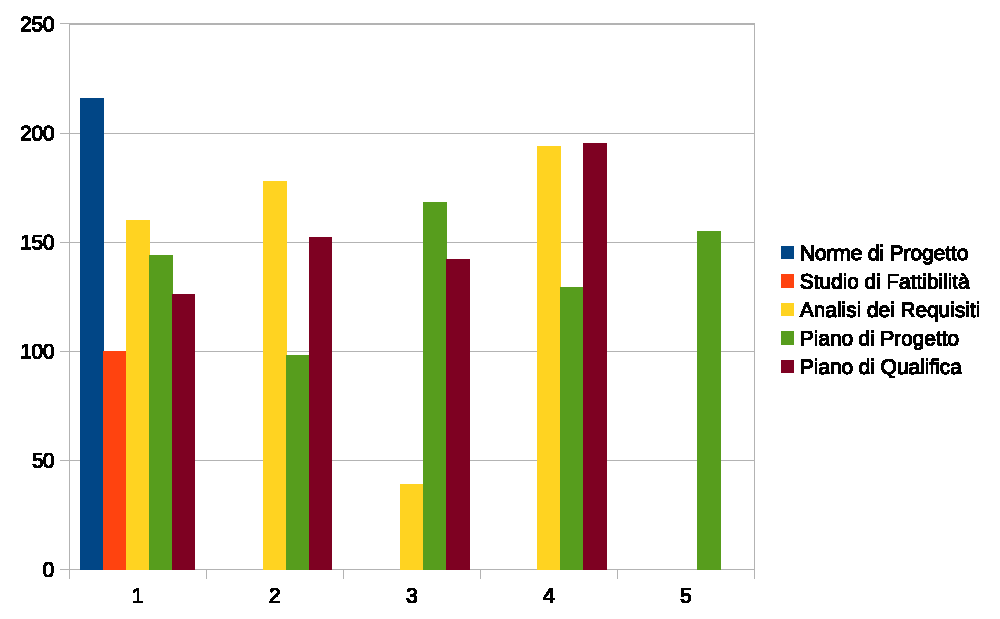
\includegraphics[width=12cm]{PianoDiQualifica/Pics/ProduttivitaDocumentazioneFaseDB.pdf}
					\caption{Produttività del processo di documentazione durante la Fase DB}
				\end{figure}
				Si può, in generale, notare un miglioramento nella produttività. Questo, probabilmente, è imputabile ai seguenti fatti:
				\begin{itemize}
					\item i componenti del \insglo{team} hanno assimilato i contenuti delle \insdoc{Norme di Progetto v1.00} e non devono continuamente far 
					riferimento ad esse;
					\item il gruppo sta imparando i comandi \LaTeX{} previsti per la stesura dei documenti e di conseguenza la stesura risulta più veloce;
					\item è stata imposta una struttura prefissata ai documenti, togliendo di conseguenza questa responsabilità dai redattori.
				\end{itemize}
				Il picco negativo nella produttività del documento \insdoc{Analisi dei Requisiti v1.00} è imputabile ai problemi avuti dagli Analisti durante 
				la loro attività: il loro lavoro infatti è stato rallentato a causa di una cattiva comprensione dei diagrammi dei casi d'uso.
		\level{3}{Processo di verifica}
			\level{4}{Livello CMM}
				L'obiettivo, fin da subito, è stato quello di realizzare un processo di verifica di qualità. La principale ragione per fare ciò è che la 
				verifica occupa una parte cospicua del progetto: di conseguenza essa è molto costosa. La si vuole rendere più efficace e allo stesso 
				tempo efficiente possibile. Per ottenere tali obiettivi si deve rendere il processo controllabile.\\
				Anche per quanto riguarda questo processo, come per quello di documentazione, siamo in grado di dire che è stato raggiunto il livello 2 
				nella scala prevista da \insglo{CMM} (nella versione 1.00 il livello 2 non è stato considerato accettabile, solo nelle versioni successive il secondo livello \insglo{CMM} viene ritenuto accettabile in quanto segno una prima gestione del processo). Il processo ha infatti superato l'iniziale stato caotico nel quale si trovava all'inizio della \insphase{Fase DB}
				(grazie, per esempio, all'introduzione di una lista di controllo per gli errori comuni o all'utilizzo sistematico di strumenti 
				automatici e di procedure). Tuttavia il \insglo{team} non può ancora affermare che il processo di verifica adottato abbia raggiunto un livello di 
				maturità 3, in quanto è stata documentata in modo accettabile solo l'attività di realizzazione del processo, e non quella di gestione 
				dello stesso.
			\level{4}{Produttività}
				Utilizzando la formula descritta all'interno del presente documento (sezione \nameref{sec:metriche}) è stata calcolata la produttività del 
				processo di verifica. Tale indice è stato calcolato in seguito a tutti i momenti di verifica previsti dal \insdoc{Piano di Progetto v1.00} per 
				la \insphase{Fase DB}. Di seguito vengono riportati i valori calcolati e una loro rappresentazione grafica.
				\begin{table}[H]
					\centering
						\begin{tabu}{| l | c | c | c | c | c | c | c |}
							\hline
								&14-17/12	&21-24/12	&27-31/12 	&01-04/01	&09-12/01	&13-16/01	&17-19/01	\\ \hline
							Produttività	&15	&9	&16	&18	&15	&14	&16\\ \hline
						\end{tabu}
					\caption{Produttività del processo di verifica durante la fase DB}
				\end{table}
				\begin{figure}[H]
					\centering
					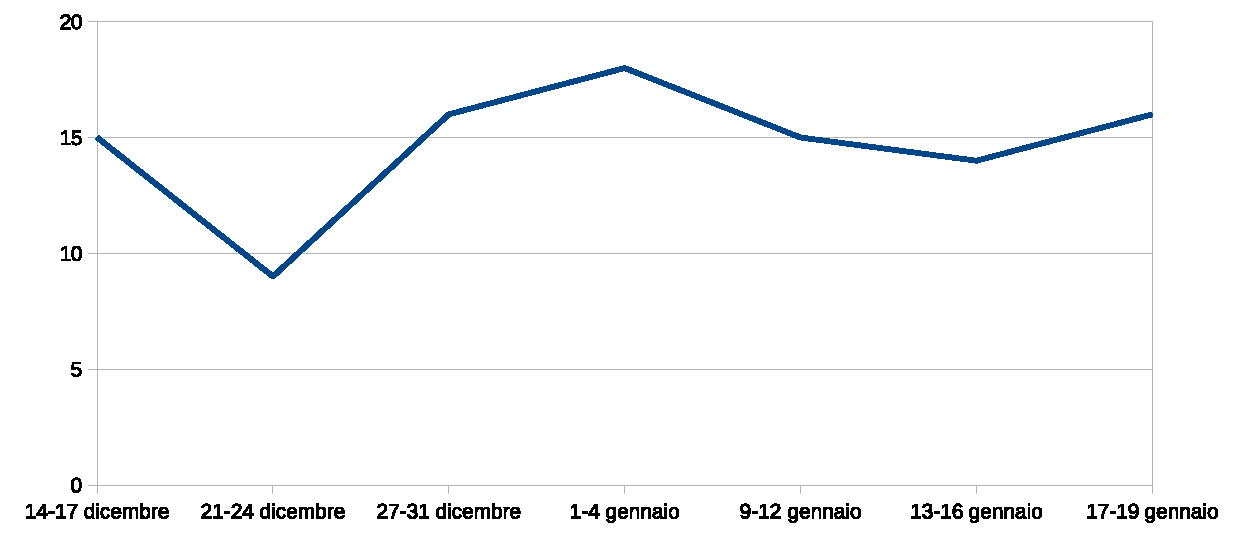
\includegraphics[width=12cm]{PianoDiQualifica/Pics/ProduttivitaVerificaFaseDB.pdf}
					\caption{Produttività del processo di verifica durante la Fase DB}
				\end{figure}
				Dai dati si può notare come la produttività del processo di verifica non sia aumentata in modo sostanziale durante la \insphase{Fase DB}, nonostante 
				i miglioramenti apportati in termini di procedure e strumenti. Probabilmente questo è dovuto ad un aumento della qualità dei prodotti 
				ispezionati di volta in volta. Infatti, i redattori si sono adeguati a perseguire con maggior rigore gli obiettivi di qualità che il \insglo{team} 
				si è imposto (e che sono descritti all'interno del presente documento), secondo il principio che la qualità è una responsabilità di tutti.
			\level{4}{Efficacia di una revisione}
				Utilizzando la formula descritta all'interno del presente documento (sezione \nameref{sec:metriche}) è stata calcolata l'efficacia delle 
				varie revisioni che sono state fatte durante la \insphase{Fase DB}. Di seguito vengono riportati i valori calcolati e una loro rappresentazione grafica.
				\begin{table}[H]
					\centering
					\begin{tabu}{| l | c | c | c | c | c | c | c |}
						\hline
							&14-17/12	&21-24/12	&27-31/12 	&01-04/01	&09-12/01	&13-16/01	&17-19/01	\\ \hline
						Efficacia	&9	&6	&7	&5	&7	&7	&8 \\ \hline
					\end{tabu}
					\caption{Efficacia delle revisioni durante la fase DB}
				\end{table}
				\begin{figure}[H]
					\centering
					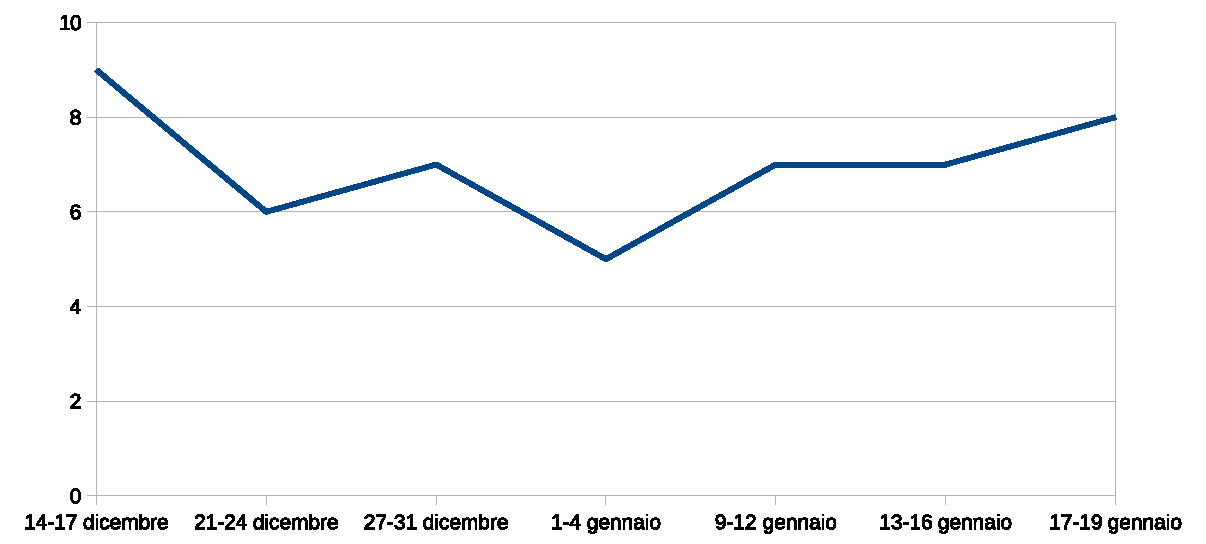
\includegraphics[width=12cm]{PianoDiQualifica/Pics/EfficaciaRevisioniFaseDB.pdf}
					\caption{Efficacia delle revisioni durante la Fase DB}
				\end{figure}
				Dal grafico sopra presentato si può notare come non vi sia stato un miglioramento tangibile dell'efficacia delle revisioni che sono 
				state fatte durante la \insphase{Fase DB}. I motivi non sono facilmente comprensibili a causa dell'inesperienza del \insglo{team}, ma si può azzardare 
				l'ipotesi che non siano stati utilizzati sufficienti strumenti in grado di automatizzare la verifica. Infatti, è molto più facile 
				aumentare l'efficacia di una revisione se questa viene fatta in modo automatico piuttosto che aumentare l'efficacia di una revisione 
				eseguita perlopiù manualmente. Il \insglo{team}, dunque, per le prossime fasi, si impegna a includere un maggior numero di strumenti di supporto 
				al processo di verifica (in particolare per quanto riguarda la verifica della documentazione).
		\level{3}{PDCA}
			In questa sezione viene riportato il grafico \insglo{PDCA} della \insphase{Fase DB}. In ascissa è rappresentato il tempo, in ordinata le attività.
			\begin{figure}[H]
				\centering
				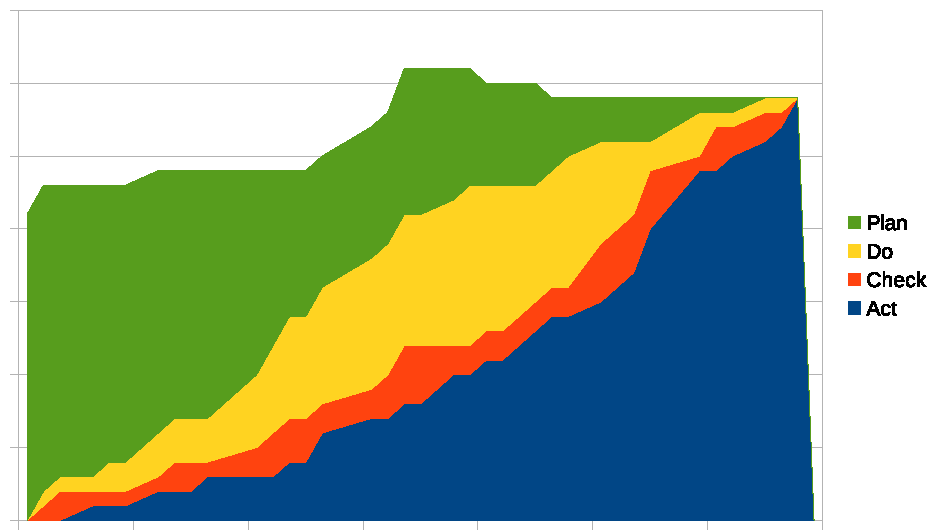
\includegraphics[width=0.6\textwidth]{PianoDiQualifica/Pics/GraficoPDCAFaseDB.pdf}
				\caption{PDCA Fase DB}
			\end{figure}
			Guardando il grafico si può notare come nella parte centrale vi sia un mutamento dei processi pianificati. Le cause di questo evento 
			inaspettato	risiedono principalmente nell'inesperienza in un'attività come la pianificazione. Inoltre ciò è stato dovuto a dei problemi 
			riscontrati dagli Analisti nella creazione dei diagrammi dei casi d'uso per il documento \insdoc{Analisi dei Requisiti v1.00}.\\
			Si può infine notare come vi sia un lieve rallentamento delle attività nella parte finale causato dalla vicinanza della sessione di esami.
